%\documentclass[german,10pt]{book}      
\usepackage{makeidx}
\usepackage{babel}            % Sprachunterstuetzung
\usepackage{amsmath}          % AMS "Grundpaket"
\usepackage{amssymb,amsfonts,amsthm,amscd} 
\usepackage{mathrsfs}
\usepackage{rotating}
\usepackage{sidecap}
\usepackage{graphicx}
\usepackage{color}
\usepackage{fancybox}
\usepackage{tikz}
\usetikzlibrary{arrows,snakes,backgrounds}
\usepackage{hyperref}
\hypersetup{colorlinks=true,
                    linkcolor=blue,
                    filecolor=magenta,
                    urlcolor=cyan,
                    pdftitle={Overleaf Example},
                    pdfpagemode=FullScreen,}
%\newcommand{\hyperref}[1]{\ref{#1}}
%
\definecolor{Gray}{gray}{0.80}
\DeclareMathSymbol{,}{\mathord}{letters}{"3B}
%
\newcounter{num}
\renewcommand{\thenum}{\arabic{num}}
\newenvironment{anmerkungen}
   {\begin{list}{(\thenum)}{%
   \usecounter{num}%
   \leftmargin0pt
   \itemindent5pt
   \topsep0pt
   \labelwidth0pt}%
   }{\end{list}}
%
\renewcommand{\arraystretch}{1.15}                % in Formeln und Tabellen   
\renewcommand{\baselinestretch}{1.15}                 % 1.15 facher
                                                      % Zeilenabst.
\newcommand{\Anmerkung}[1]{{\begin{footnotesize}#1 \end{footnotesize}}\\[0.2cm]}
\newcommand{\comment}[1]{}
\setlength{\parindent}{0em}           % Nicht einruecken am Anfang der Zeile 

\setlength{\textwidth}{15.4cm}
\setlength{\textheight}{23.0cm}
\setlength{\oddsidemargin}{1.0mm} 
\setlength{\evensidemargin}{-6.5mm}
\setlength{\topmargin}{-10mm} 
\setlength{\headheight}{0mm}
\newcommand{\identity}{{\bf 1}}
%
\newcommand{\vs}{\vspace{0.3cm}}
\newcommand{\noi}{\noindent}
\newcommand{\leer}{}

\newcommand{\engl}[1]{[\textit{#1}]}
\parindent 1.2cm
\sloppy

         \begin{document}  \setcounter{chapter}{9}

\chapter{Landkarten und der metrische Tensor}
% Kap 10
\label{chap_Landkarte}

\info{Thomas Filk}{28.03.2024}%
Die fundamentale dynamische Gr\"o\ss e in der Allgemeinen Relativit\"atstheorie
ist die Metrik bzw.\ der metrische Tensor, oft geschrieben als $g_{\mu \nu}(x)$, wobei
$x$ die Punkte der Raumzeit parametrisiert. 
In der Mathematik, insbesondere der Differentialgeometrie, geht der
Definition dieses Feldtensors
eine von einer Einbettung unabh\"angige Definition einer Mannigfaltigkeit voraus.
Dies wird hier umgangen, auch wenn das Konzept der Karte und des Atlas einer
solchen Beschreibung schon sehr nahe kommen.  

In diesem Kapitel wird der Begriff des metrischen Feldtensors anhand von 
Landkarten\index{Landkarten|(}
veranschaulicht. Landkarten sind L\"osungen des Problems, Ausschnitte einer Kugeloberfl\"ache
in einer Ebene darzustellen. Das ist mit l\"angentreuen Darstellungen, die gr\"o\ss ere Bereiche der
Erdoberfl\"ache wiedergeben, nicht m\"oglich. Besonders deutlich wird dies an Weltkarten. 
Hier kommt es immer zu deutlichen Verzerrungen und die Kunst besteht darin, die gr\"obsten Verzerrungen
in solche Bereiche zu legen, die f\"ur die konkrete Anwendung weniger relevant sind. Au\ss erdem ist man
man je nach Anwendung daran interessiert, unterschiedliche Dinge auf einer Karte
invariant zu lassen. Es gibt winkeltreue bzw.\ formtreue Darstellungen der Kugeloberfl\"ache, die
aber die Fl\"achen unterschiedlich skalieren, und es gibt fl\"achentreue Darstellungen, die
aber die Formen sehr verzerren. Und dann gibt es nat\"urlich sehr viele Optionen
dazwischen. 

Bei einer Weltkarte kommen neben den Verzerrungen noch sogenannte Koordinatensingularit\"aten
hinzu.\index{Koordinatensingularit\"at} 
Dabei handelt es sich um singul\"are Punkte oder Linien (typischerweise am Rand der
Karte, z.B.\ an den Polen), bei denen die Bijektivit\"at zwischen der Karte und dem dargestellten
Gebiet verloren geht. Solche Koordinatensingularit\"aten treten immer dann auf, wenn die
Topologie der darzustellenden Mannigfaltigkeit -- hier der Kugeloberfl\"ache -- nicht mit der 
Topologie der darstellenden Mannigfaltigkeit -- hier dem zusammenh\"angenden Ausschnitt einer euklidischen
Ebene -- \"ubereinstimmt. Das Gebiet selbst hat nat\"urlich keine Singularit\"at -- die Oberfl\"ache einer
Kugel ist glatt -- sondern nur die Karte. In der Allgemeinen Relativit\"atstheorie treten solche
Koordinatensingularit\"aten ebenfalls auf (z.B.\ ist der Horizont eines Schwarzen Lochs in der
\"ublichen Darstellung der Schwarzschild-Koordinaten eine Koordinatensingularit\"at). Allerdings
gibt es auch L\"osungen der Einstein'schen Gleichungen mit wirklichen (physikalischen) Singularit\"aten,
z.B.\ das Zentrum eines Schwarzen Lochs, bei dem die Gezeitenkr\"afte unendlich werden. Es ist
nicht immer leicht, eine Koordinatensingularit\"at von einer physikalischen Singularit\"at zu unterscheiden.

In den kommenden ersten Abschnitten wird zun\"achst der Begriff der Metrik anhand eines ortsabh\"angigen
Kartenma\ss stabs erl\"autert. Der Rest des Kapitels besteht im Wesentlichen aus Beispielen.

\section{Ortsabh\"angige Landkartenma\ss st\"abe}
\label{sec_ortsabhaengig}

Eine Landkarte enth\"alt\index{Massstab@Ma\ss stab} 
gew\"ohnlich eine Ma\ss stabsangabe, beispielsweise eine
Wanderkarte 1:25\,000 oder eine Stra\ss enkarte 1:250\,000. Das bedeutet, eine
L\"angeneinheit auf der Karte (z.B.\ ein Zentimeter) entspricht 25\,000 bzw.\ 250\,000 dieser 
L\"angeneinheiten in Wirklichkeit, das sind somit 250\,m bzw.\ 2,5\,km.  
Eine Ma\ss stabsangabe setzt somit eine Distanz auf der Karte mit einer Distanz auf der
von der Karte dargestellten Mannigfaltigkeit in Beziehung. Nichts anderes macht der metrische
Tensor in der Differentialgeometrie, allerdings kommt hier eine Komplikation hinzu, die man
auch schon bei Landkarten findet: die Orts- und Richtungsabh\"angigkeit des Ma\ss stabs.

Der Ma\ss stab einer Landkarte kann nicht \"uberall derselbe sein, und wenn diese
Landkarte gro\ss e Gebiete darstellt oder sehr pr\"azise sein soll
(z.B.\ eine Seekarte f\"ur die Schifffahrt), sollte angegeben sein, wie die Korrektur zum
allgemeinen Ma\ss stab aussieht. Bei groben Weltkarten werden diese Korrekturen oft nicht
angegeben, obwohl sie offensichtlich vorhanden sind. Abbildung \ref{fig_Zylinder} zeigt eine Weltkarte
in einer sogenannten\index{Zylinderprojektion!quadratische} 
quadratischen Zylinderprojektion. Die $x$- und $y$-Achse entsprechen
den L\"angen- und Breitengraden. Der Abstand zwischen zwei eingezeichneten L\"angengraden am
\"Aquator betr\"agt rund 556\,km (die Karte ist in $5^\circ$-Abschnitte unterteilt). Dieser
Abstand verringert sich mit dem Breitengrad $\theta$ (vom \"Aquator aus gerechnet) um einen Faktor
$\cos \theta$, betr\"agt also am 60.\ Breitengrad (das entspricht der H\"ohe von Helsinki) nur noch die H\"alfte.   

\begin{SCfigure}[30][htb]
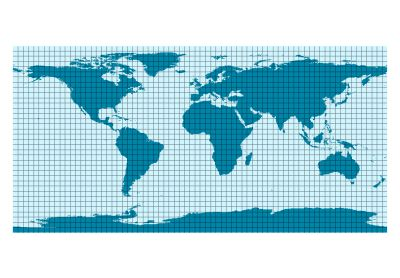
\includegraphics[trim= 0cm 1.0cm 0.3cm 1.0cm,clip,width=0.55\textwidth]{./Bilder/Zylinderprojektion.jpg}
\caption{\label{fig_Zylinder}%
Eine Weltkarte in rechteckiger Form. Gleiche Breiten- und
L\"angengrade entsprechen gleichen Abst\"anden auf der Karte. Es ist offensichtlich, dass sich
der Ma\ss stab in Ost-West-Richtung in der N\"ahe der Pole \"andert. Die Netzeinteilung ist
in $5^\circ$-Schritten. Am \"Aquator entspricht einer Einheit rund 556\,km, beim $60$.\ Breitengrad
ist es nur noch die H\"alfte. (Quelle \cite{WikiNetz})}  
\end{SCfigure}
 
Der Ma\ss stab einer solchen Karte h\"angt also sowohl vom Ort ab, an dem man 
die Beziehung zwischen Karte und Erdoberfl\"ache bestimmen m\"ochte, als auch von der
Richtung. Bei der in Abb.\ \ref{fig_Zylinder} verwendeten Darstellung \"andert sich der
Ma\ss stab nicht f\"ur Punkte auf demselben L\"angengrad, also in Nord-S\"ud-Richtung: 
Gleiche Breitengraddifferenzen entsprechen auch
gleichen Abst\"anden. Es \"andern sich lediglich die Abst\"ande zwischen den L\"angengraden 
als Funktion vom Breitengrad.\index{Laengengrad@L\"angengrad}\index{Breitengrad}  

In dieser Darstellung wirken somit L\"ander am n\"ordlichen Rand oder auch
die Antarktis am s\"udlichen Rand sehr in die Breite gestreckt. Andere Darstellungen versuchen
diese Problematik zu beheben: Beispielsweise findet man bei der\index{Mercator-Projektion} 
Mercator-Projektion (Abschnitt \ref{sec_Mercator}, Abb.\ \ref{fig_Mercator}) 
dieselbe Streckung auch in Nord-S\"ud-Richtung, sodass die Proportionen in der Form wieder stimmen,
allerdings wirken nun Gebiete in Poln\"ahe wesentlich gr\"o\ss er als in \"Aquatorn\"ahe, d.h.\ diese
Karten skalieren die Fl\"achen ungleich. Andere Projektionen, beispielsweise die\index{Lambert-Projektion} 
Lambert-Projektion (Abschnitt \ref{sec_Lambert}, Abb.\ \ref{fig_Lambert}),
behalten die Fl\"acheninhalte bei, sie stauchen aber zus\"atzlich die Abst\"ande  in Nord-S\"ud-Richtung,
sodass die Gebiete noch flacher aussehen. Wir behandeln diese Darstellungen in den
sp\"ateren Abschnitten. Hier soll als wesentlicher Punkt festgehalten werden, dass bei Landkarten
die Ma\ss st\"abe (a) vom Ort abh\"angen k\"onnen und (b) richtungsabh\"angig sein k\"onnen. 
Au\ss erdem muss die Streckung bzw.\ Stauchung nicht in Ost-West- oder Nord-S\"udrichtung erfolgen,
sondern kann auch \glqq schr\"ag\grqq\ verlaufen. Der folgende Abschnitt beschreibt, wie man
diese Art von Verzerrung lokal beschreiben kann und wie der Kartenma\ss stab mit dem metrischen
Tensor zusammenh\"angt. 

\section{Beschreibung einer Ellipse} 

In einem zweidimensionalen kartesischen
Koordinatensystem l\"asst sich eine Ellipse algebraisch beispielsweise durch die folgenden
zwei Formen darstellen:\index{Ellipse}
\begin{equation}
\label{eq_Ellipse1}
            \pmb{x}(\varphi) = r (a \cos \varphi, b \sin \varphi) ~,~~  \varphi \in [0,2\pi)
            \hspace{1cm} {\rm und} \hspace{1cm}
             \frac{x^2}{a^2} + \frac{y^2}{b^2} = r^2 \, .
\end{equation}
Die \"Aquivalenz dieser beiden Darstellungen erkennt man sofort, wenn man f\"ur $x$ und $y$ in
der rechten Darstellung die Ausdr\"ucke der linken Darstellung ($x=ar\cos \varphi$ und $y=br\sin \varphi$)
einsetzt. Aus beiden Darstellungen wird deutlich, dass es sich bei einer Ellipse um einen
gestauchten oder gestreckten Kreis handelt: Multipliziert man die $y$-Komponente mit $a/b$ erh\"alt
man die Gleichung eines Kreises. Sofern $a>b$ gilt, sind $ar$ und $br$ die gro\ss e und die kleine 
Halbachse der Ellipse. Der zus\"atzliche Parameter $r$ hat folgenden Grund:
$x$ und $y$ sollen die Dimension einer L\"ange haben (hier handelt es sich um Abst\"ande auf
einer Karte), ebenso soll $r$ die Dimension einer L\"ange haben (hier handelt es sich um einen
Abstand auf der Erdkugel); die beiden Parameter $a$ und $b$ sollen dimensionslose
Skalierungsfaktoren sein. Beispielsweise w\"aren bei einer normalen Karte mit dem
Ma\ss stab 1:25\,000 diese Parameter $a=b=1/25\,000$. 

Die Halbachsen sind entlang der Koordinatenachsen ausgerichtet.
F\"ur eine allgemeine Darstellung einer Ellipse kann man die Koordinaten noch um den Winkel $\alpha$
drehen, d.h.
\begin{equation}
\label{eq_Ellipse2}
        x \mapsto  x\cos \alpha  - y \sin \alpha   \hspace{1cm} {\rm und} \hspace{1cm}
        y \mapsto  x\sin \alpha + y \cos \alpha    
\end{equation}
und erh\"alt die Form:
\begin{equation}
\label{eq_Ellipse3}
             \frac{x^2 \cos^2 \alpha + y^2 \sin^2 \alpha - 2xy \cos \alpha \sin \alpha}{a^2} + 
             \frac{x^2 \sin^2 \alpha + y^2 \cos^2 \alpha + 2xy \cos \alpha \sin \alpha}{b^2} = r^2 
\end{equation}
oder
\begin{equation}
\label{eq_Ellipse4}
            g_{11} x^2 +  (g_{12}+g_{21})  xy + g_{22} y^2 = r^2 
\end{equation}
mit
\begin{equation}
\label{eq_Ellipse5}
            g_{11} = \frac{\cos^2 \alpha}{a^2} + \frac{\sin^2 \alpha}{b^2}   \hspace{1cm}
            g_{22} = \frac{\sin^2 \alpha}{a^2} + \frac{\cos^2 \alpha}{b^2}   \hspace{1cm}
            g_{12} = g_{21} = \left( \frac{1}{b^2} - \frac{1}{a^2}  \right) \cos \alpha \sin \alpha \, .
\end{equation}
Aus dieser Darstellung finden wir:
\begin{equation}
\label{eq_Ellipse6}
        g_{11}+g_{22} = \frac{1}{a^2} + \frac{1}{b^2} \hspace{1cm} {\rm und} \hspace{1cm}
        g_{11} g_{22} - g_{12}^2 = \frac{1}{a^2\,b^2}  \, .
\end{equation}
Wir erkennen somit: Gleichung \ref{eq_Ellipse4} l\"asst sich in der Form
\begin{equation}
                  \pmb{x}^T \cdot g \pmb{x} = ( x,y) 
                  \left( \begin{array}{cc} g_{11} & g_{12} \\ g_{21} & g_{22} \end{array} \right)
                  \left( \begin{array}{c} x \\ y \end{array} \right) =r^2
\end{equation}
schreiben, wobei Gl.\ \ref{eq_Ellipse6} zum Ausdruck bringt, dass die Matrix $g$ die
Eigenwerte $\lambda_1=1/a^2$ und $\lambda_2=1/b^2$ hat (in Gl.\ \ref{eq_Ellipse6} steht links
die Spur -- also die Summe der Eigenwerte -- und rechts die Determinante von $g$ -- also das
Produkt der Eigenwerte). Die Bilinearform in Gl.\ \ref{eq_Ellipse3} bzw.\ \ref{eq_Ellipse4} wird durch
eine Drehung um $-\alpha$ diagonalisiert und auf die Form in Gl.\ \ref{eq_Ellipse1} gebracht (da
kam sie auch schlie\ss lich einmal her). 

\section{Tissot-Indikatrix und die Metrik} 
\label{sec_Tissot}

Wie wir in Abschnitt \ref{sec_ortsabhaengig} gesehen haben, ben\"otigen die meisten
Landkarten (insbesondere alle Landkarten, die ein gro\ss es Gebiet der Erdkugel darstellen)
einen ortsabh\"angigen Ma\ss stab. Dieser Ma\ss stab bringt zum Ausdruck, wie
ein Kreis auf der Erdkugel in der Karte wiedergegeben wird, wobei diese Darstellung
in f\"uhrender Ordnung (d.h., wenn dieser Kreis klein ist im Vergleich zu der Skala, auf
der sich der Ma\ss stab ver\"andert) den Kreis zu einer Ellipse verformt. Einen ortsabh\"angigen   
Ma\ss stab k\"onnen wir also dadurch kennzeichnen, dass wir an jedem Punkt der Karte die
Parameter $g_{ij}$ angeben, die nach Gl.\ \ref{eq_Ellipse4} eine Ellipse charakterisieren. Genau
dies ist aber der metrische Feldtensor. Das soll in diesem Abschnitt erl\"autert werden. 

\begin{figure}[htb]
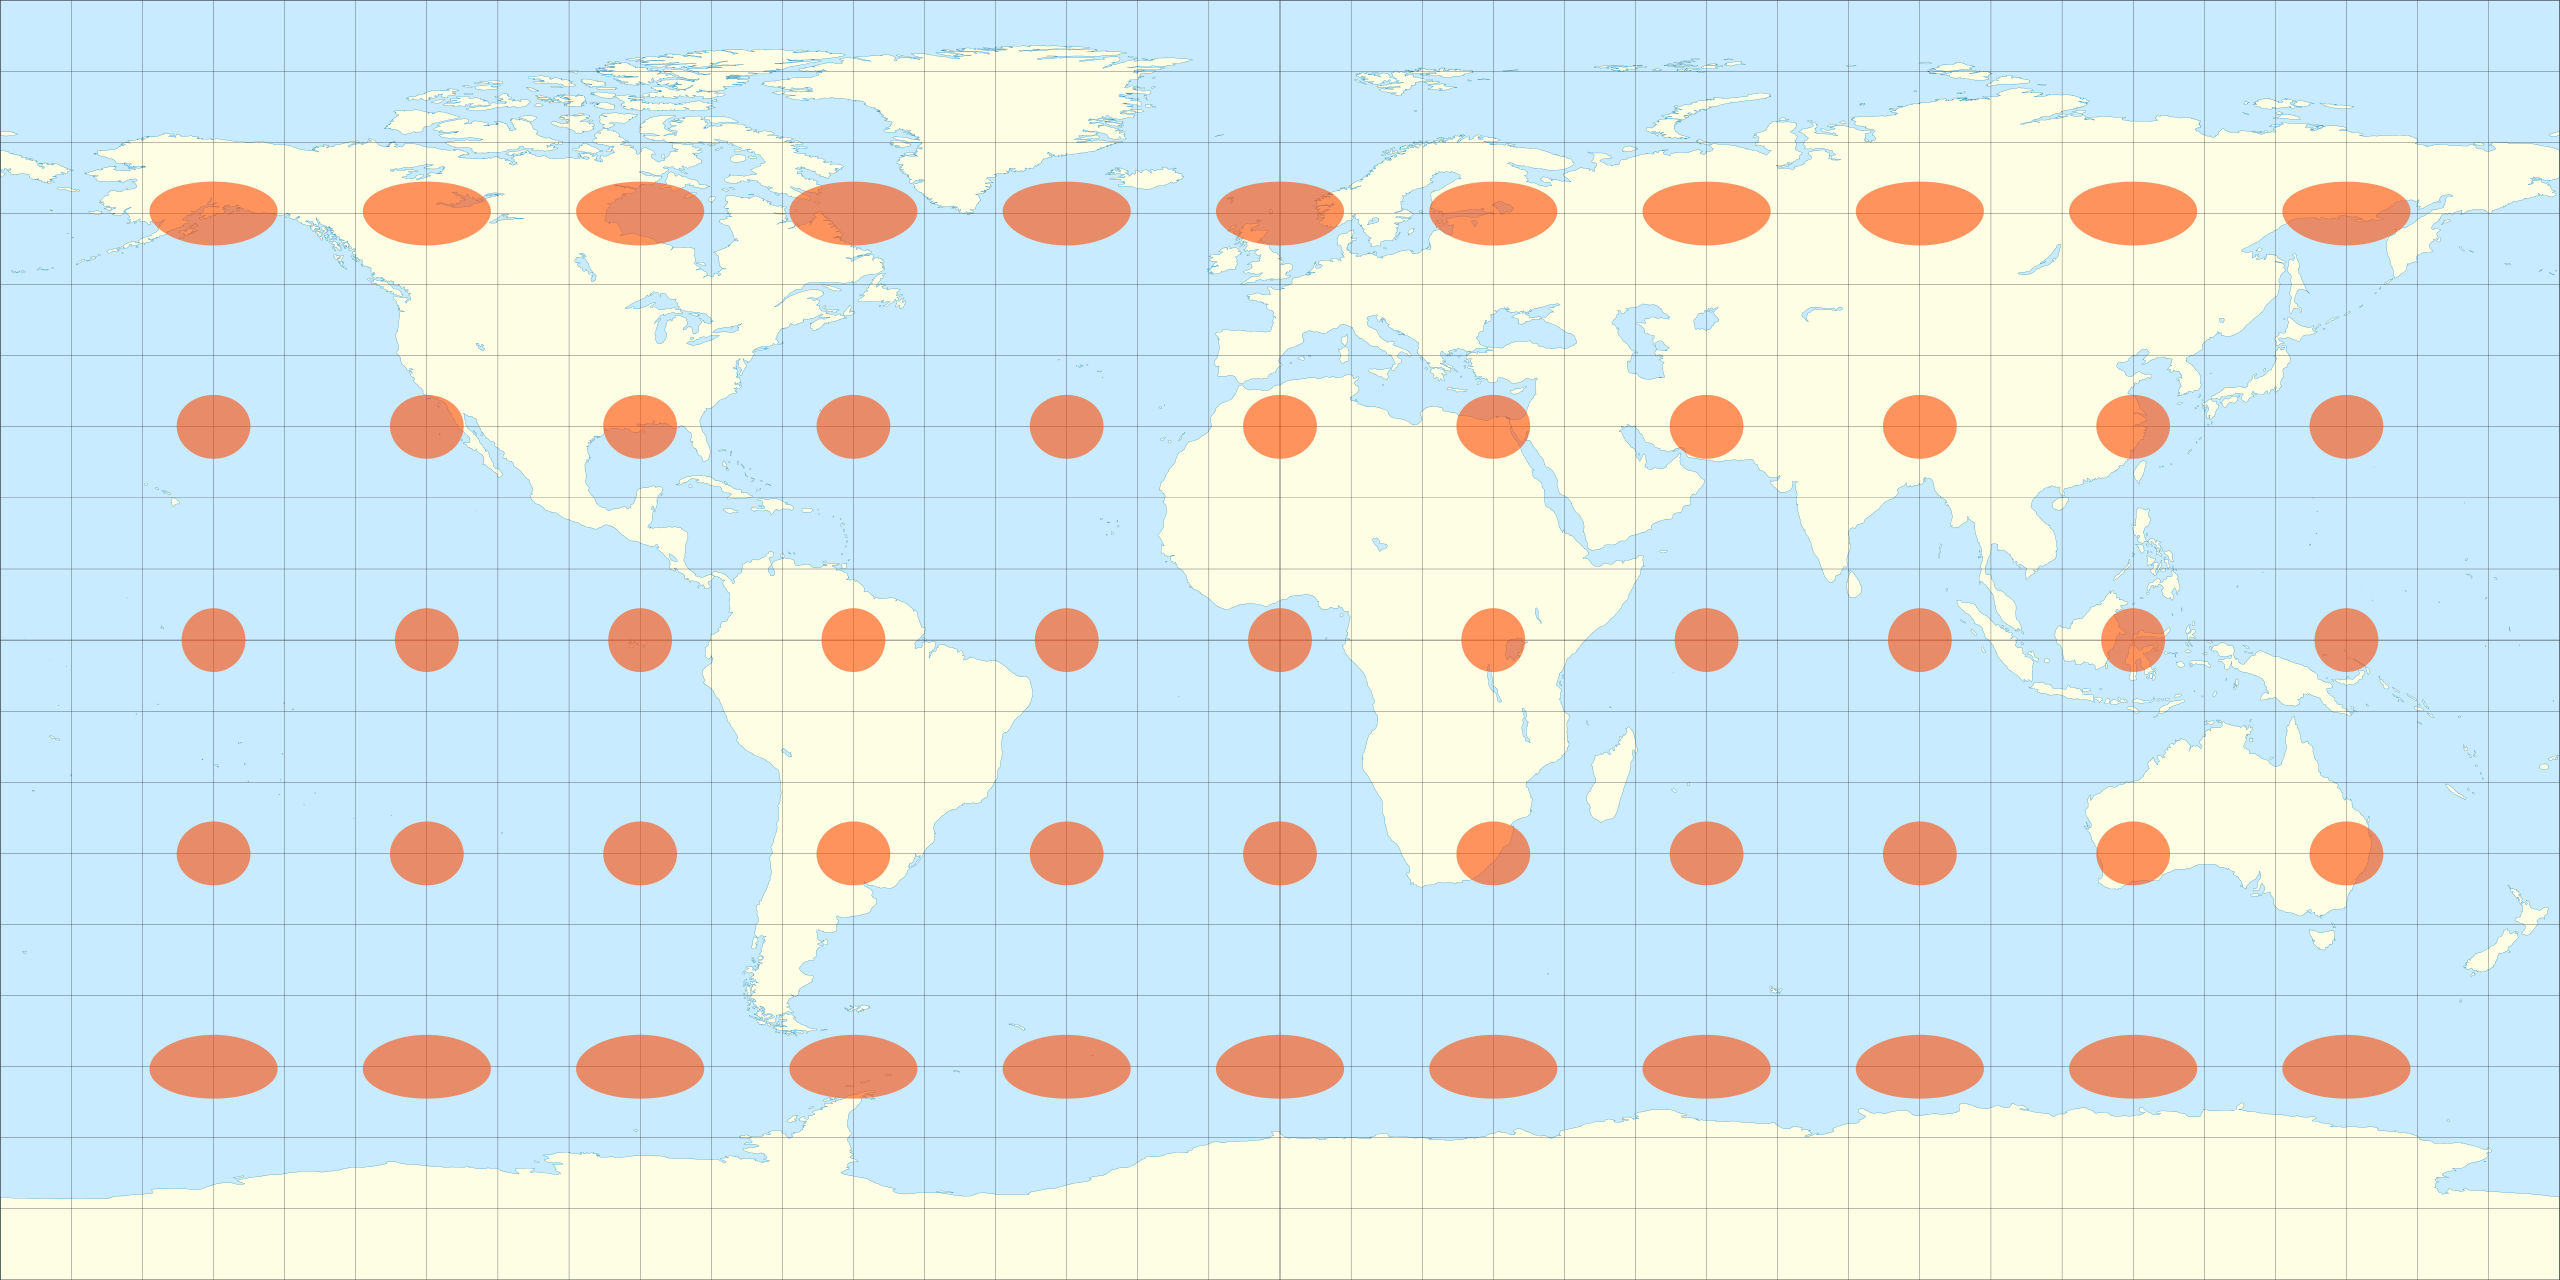
\includegraphics[width=\textwidth]{./Bilder/Tissot_rectangle.png}
\caption{\label{fig_Tissot1}\index{Tissot'sche Indikatrix}%
Tissot'sche Indikatrix zur quadratischen Zylinderprojektion. Die Ellipsen entsprechen den
Darstellungen von Kreisen auf der Kugeloberfl\"ache in der Karte (Quelle \cite{WikiTissot}).}
\end{figure}


Abbildung \ref{fig_Tissot1} zeigt nochmals eine quadratische Zylinderprojektion, bei der die
Abschnitte entlang der L\"angengrade (also in Nord-S\"ud-Richtung)
einen konstanten Abstand haben, d.h., hier werden
die L\"angen- und Breitengrade in einem kartesischen Koordinatensystem dargestellt. 
Wie schon besprochen, f\"uhrt diese Darstellung zu einer Verzerrung in Ost-West-Richtung
in Abh\"angigkeit vom Breitengrad: Je n\"aher der Breitengrad an den Polen ist, umso
gr\"o\ss er ist die Dehnung im Vergleich zum \"Aquator, wo der Ma\ss stab in alle Richtungen
derselbe ist. Ein hypothetischer Kreis auf der Erde (in diesem Fall ein Kreis mit einem 
Radius von rund $r=500$\,km) wird in der Karte durch eine Ellipse wiedergegeben. Diese
Ellipse entartet am \"Aquator zu einem Kreis (dort sind die Ma\ss st\"abe in alle
Richtungen gleich) und wird in Ost-West-Richtung gestreckt, je weiter man sich vom 
\"Aquator entfernt. Auf dem 60.\ Breitengrad ist die gro\ss e Halbachse bereits doppelt so gro\ss\
wie die kleine Halbachse. Beide Halbachsen entsprechen jedoch immer noch auf der
Erdkugel einer Strecke von 500\,km. Man bezeichnet diese Darstellung des ortsabh\"angigen
Kartenma\ss stabs auch als Tissot'sche Indikatrix. Wir nennen die Kartenabbildung von Kreisen auf der
Kugeloberfl\"ache dann Tissot-Ellipsen.\index{Tissot-Ellipse} 
Die Charakterisierung einer Tissot-Ellipse an einem
bestimmten Ort auf der Karte durch die Parameter der Ellipse in Form der Matrix $g_{ij}$
bezeichnet man als metrischen Feldtensor.\index{Feldtensor, metrischer} 
\glqq metrisch\grqq\ bedeutet, dass dieses
Objekt die Ma\ss st\"abe zur Bestimmung von Entfernungen kodiert, \glqq Feld-\grqq\ bedeutet,
dass dieses Objekt an jedem Ort definiert und von Ort zu Ort verschieden sein kann, und 
\glqq Tensor\grqq\ bedeutet, dass es sich um eine Matrix handelt, die die Richtungsabh\"angigkeit
angibt.\footnote{Streng genommen bezieht sich \glqq Tensor\grqq\ darauf, wie sich die Elemente von
$g_{ij}$ unter Koordinatentransformationen ver\"andern, das soll hier aber nicht weiter
vertieft werden.} 

Zur Bestimmung der Parameter $a$ und $b$ k\"onnen wir folgenderma\ss en vorgehen (ein
allgemeines Verfahren, wie man aus einer Parameterdarstellung der Kugeloberfl\"ache diese
Parameter gewinnt, beschreiben wir
in Abschnitt \ref{sec_Parameter}). Die Karte habe eine Breite $B$ (hier ungef\"ahr $B=154$\,mm)
und eine H\"ohe $H=B/2$ (da die Ost-West-Richtung in 360 Grade, die Nord-S\"ud-Richtung
aber nur in 180 Grade unterteilt ist, und beide Richtungen dieselbe Skala haben sollen). 
Der Erdumfang am \"Aquator betr\"agt $U=40\,000$\,km 
(wir gehen hier von einer idealen Kugel mit dieser L\"ange eines Gro\ss kreises aus).
Allgemein: Wenn eine Strecke auf einer Kugel (hier der Umfang) die L\"ange $U$ hat und auf einer Karte 
im Abstand $B$ (hier der Breite der Karte) dargestellt wird, 
dann hat die Karte einen Ma\ss stab von $1:U/B$, hier ungef\"ahr $1:260\,000\,000$.  

Entfernt man sich nun vom \"Aquator in Richtung der Pole \"andert sich
dieser Ma\ss stab in Ost-West-Richtung (d.h.\ f\"ur Punkte auf demselben Breitengrad) 
und der Abstand zwischen zwei L\"angengraden bei einem Breitengrad $\theta$ wird
um den Faktor $\cos \theta$ k\"urzer. Wir erhalten also f\"ur den Ma\ss stab in Ost-West-Richtung am
Breitengrad $\theta$ den Wert $(U/B) \cos \theta$. Damit folgt:
\begin{equation}
           a(\theta,\varphi) = \frac{B}{U\cos \theta} \approx \frac{1}{260\,000\,000 \cos \theta} \hspace{1cm} {\rm und}
           \hspace{1cm}  b(\theta,\varphi) = \frac{B}{U} \approx \frac{1}{260\,000\,000}  \, .  
\end{equation}
Diese Parameter h\"angen nicht von $\varphi$ (dem L\"angengrad) ab sondern nur vom Breitengrad.
Der Ma\ss stab am \"Aquator f\"ur obige Karte (mit der Breite 154\,mm) w\"are somit $1:260\,000\,000$. 
Der metrische Feldtensor w\"are
\begin{equation}
               g = \left( \begin{array}{cc}   \left( \frac{U}{B} \right)^2  \cos^2 \theta & 0 \\ 0 & \left( \frac{U}{B} \right)^2
               \end{array} \right) \, .
\end{equation}
Man erkennt, dass $g_{11}$ bei $\theta=\pm 90^\circ$ (also an den Polen) verschwindet. Hierbei
handelt es sich um eine typische Koordinatensingularit\"at,\index{Koordinatensingularit\"at} 
bei der ein einzelner Punkt
(der Nord- bzw.\ der S\"udpol) auf eine ganze Achse (den oberen bzw.\ unteren Rand der Karte)
abgebildet wird. Der Nord- bzw.\ S\"udpol sind auf der Kugel nat\"urlich vollkommen regul\"are
Punkte. 

\begin{SCfigure}[30][htb]
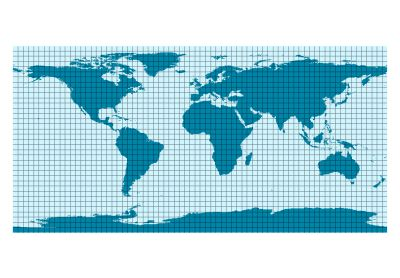
\includegraphics[trim= 0cm 1.0cm 0.3cm 1.0cm,clip,width=0.6\textwidth]{./Bilder/Zylinderprojektion.jpg}
\thicklines
\begin{picture}(0,0)(250,-50)
\qbezier(33,50)(80,85)(123,57)
\qbezier(33,50)(78,53.5)(123,57)
\end{picture}
\caption{\label{fig_Zylinder2}%
Die k\"urzeste Verbindung auf der Kugeloberfl\"ache zwischen zwei Punkten (z.B.\ Frankfurt und
San Francisco) erscheint auf einer Weltkarte als gekr\"ummte Linie. Allerdings bedarf es weniger
Tissot-Ellipsen, um diese gekr\"ummte Linie zu \"uberdecken als bei der geraden 
Verbindungslinie. (Abbildungsquelle \cite{WikiNetz})}  
\end{SCfigure}
 
\section{Parameterdarstellungen}
\label{sec_Parameter}

Unter einer Parameterdarstellung\index{Parameterdarstellung} 
einer (offenen Teilmenge einer) 2-dimensionalen Mannigfaltigkeit 
(z.B.\ einer Kugeloberfl\"ache), eingebettet in den 3-dimensionalen Raum, versteht man eine Abbildung 
der Form $(u,v) \mapsto \pmb{x}(u,v)$, wobei diese Abbildung lokal bijektiv sein soll.
Wir betrachten zun\"achst nochmals das Beispiel der Kugeloberfl\"ache, die durch die L\"angen- und
Breitengrade parametrisiert wird. 

Eine Kugel l\"asst sich in Kugelkoordinaten\index{Kugelkoordinaten} 
durch die beiden Winkel $\theta$ und $\varphi$ beschreiben:
\begin{equation}
          \pmb{x}(\theta,\varphi) = (R \cos \varphi \cos \theta, R \sin \varphi \cos \theta, R \sin \theta) \, .
\end{equation}
Im Gegensatz zur \"ublichen Wahl von Kugelkoordinaten wurde hier die Parametrisierung
so gew\"ahlt, dass der Winkel $\theta=0$ dem \"Aquator entspricht und $\theta = \pm \frac{\pi}{2}$ dem
Nord- bzw.\ S\"udpol. $\varphi$ kann die Werte $-\pi$ bis $+\pi$ annehmen, wobei $\varphi=0$
den $0$-Meridian bezeichnet. Damit entsprechen $\theta$ und $\varphi$ dem Breiten- bzw.\ L\"angengrad. 
$R$ ist der Radius der Kugel, bei der Erde ist somit $R=40\,000$\,km.  

Eine sehr kleine (infinitesimale) Verschiebung $\Delta \pmb{x}$ auf der Erdkugel, bedeutet f\"ur
die L\"angen- und Breitengrade:
\begin{equation}
       \Delta \pmb{x} = 
       \frac{\partial \pmb{x}}{\partial \theta} \Delta \theta + \frac{\partial \pmb{x}}{\partial \varphi} \Delta \varphi \, ,
\end{equation}
bzw.
\begin{equation}
\label{eq_gthetaphi}
      ( \Delta \pmb{x})^2 = 
       \left( \frac{\partial \pmb{x}}{\partial \theta} \cdot \frac{\partial \pmb{x}}{\partial \theta} \right)
       ( \Delta \theta)^2 + 2 \left( \frac{\partial \pmb{x}}{\partial \varphi} \cdot \frac{\partial \pmb{x}}{\partial \theta} \right)
       \Delta \theta \, \Delta \varphi + \left( \frac{\partial \pmb{x}}{\partial \varphi}\cdot \frac{\partial \pmb{x}}{\partial \varphi}\right)
          (\Delta \varphi )^2 \, .
\end{equation}
Durch Vergleich mit Gl.\ \ref{eq_Ellipse4} erkennen wir die folgenden Beziehungen:
\begin{equation}
       g_{\theta \theta} =   \left( \frac{\partial \pmb{x}}{\partial \theta} \cdot \frac{\partial \pmb{x}}{\partial \theta} \right)
       \hspace{1cm}
       g_{\theta \varphi} = g_{\varphi \theta} =  \left( \frac{\partial \pmb{x}}{\partial \varphi} \cdot \frac{\partial \pmb{x}}{\partial \theta} \right)
       \hspace{1cm}
       g_{\varphi \varphi} = \left( \frac{\partial \pmb{x}}{\partial \varphi}\cdot \frac{\partial \pmb{x}}{\partial \varphi}\right)  \, .
\end{equation}
Berechnen wir die beiden Vektoren
\begin{equation}
       \frac{\partial \pmb{x}}{\partial \theta} = R (- \cos \varphi \sin \theta, - \sin \varphi \sin \theta , \cos \theta)
       \hspace{0.8cm} {\rm und} \hspace{0.8cm} 
       \frac{\partial \pmb{x}}{\partial \varphi} = R (- \sin \varphi \cos \theta, \cos \varphi \cos \theta , 0)
\end{equation}
so folgt:
\begin{equation}
         g_{\theta \theta} = R^2  \hspace{1cm}   g_{\theta \varphi} = g_{\varphi \theta} = 0 
         \hspace{1cm}  g_{\varphi \varphi} = R^2 \cos^2 \theta \, .
\end{equation}
Damit haben wir bez\"uglich der Parametrisierung durch die L\"angen- und Breitengrade den metrischen
Feldtensor gefunden. Allerdings haben wir in Abschnitt \ref{sec_Tissot} die Parametrisierung durch einen
Ma\ss stab auf unserer Karte angeben, d.h.\ die $x$- und $y$-Koordinaten auf der Karte. Wir m\"ussen also noch
die Beziehungen zwischen den L\"angen- und Breitengraden und den $x$- und $y$-Koordinaten der Karte
finden. Die Breite $B$ der Karte entspricht einem Vollkreis von $360^\circ$ oder $2 \pi$, daher folgt
\begin{equation}
\label{eq_Beztheta_z1}
         \varphi = \frac{2\pi}{B} x  \hspace{0.5cm} {\rm und} \hspace{0.5cm} 
         \theta = \frac{2\pi}{B} y \hspace{1cm} {\rm bzw.} \hspace{1cm}
        \Delta \varphi = \frac{2\pi}{B} \Delta x \hspace{0.5cm} {\rm und} \hspace{0.5cm}  
        \Delta \theta = \frac{2\pi}{B} \Delta y  \, .
\end{equation}
Setzen wir diese Beziehungen in Gl.\ \ref{eq_gthetaphi} ein und nutzen aus, dass $U=2\pi R$, folgen die
Beziehungen aus Abschnitt \ref{sec_Tissot}. 

Parametrisieren wir die Kugeloberfl\"ache (oder ganz allgemein eine 2-dimensionale Mannigfaltigkeit
im 3-D-Raum) in der Form $\pmb(u,v)$, dann folgt
\begin{equation}
       \Delta \pmb{x} = 
       \frac{\partial \pmb{x}}{\partial u} \Delta u + \frac{\partial \pmb{x}}{\partial v} \Delta v \, ,
\end{equation}
bzw.
\begin{equation}
\label{eq_g_uv}
      ( \Delta \pmb{x})^2 = 
       \left( \frac{\partial \pmb{x}}{\partial u} \cdot \frac{\partial \pmb{x}}{\partial u} \right)
       ( \Delta u)^2 + 2 \left( \frac{\partial \pmb{x}}{\partial u} \cdot \frac{\partial \pmb{x}}{\partial v} \right)
       \Delta u \, \Delta v + \left( \frac{\partial \pmb{x}}{\partial v}\cdot \frac{\partial \pmb{x}}{\partial v}\right)
          (\Delta v)^2 
\end{equation}
und somit:
\begin{equation}
       g_{u u} =   \left( \frac{\partial \pmb{x}}{\partial u} \cdot \frac{\partial \pmb{x}}{\partial u} \right)
       \hspace{1cm}
       g_{u v} = g_{v u} =  \left( \frac{\partial \pmb{x}}{\partial u} \cdot \frac{\partial \pmb{x}}{\partial v} \right)
       \hspace{1cm}
       g_{v v} = \left( \frac{\partial \pmb{x}}{\partial v}\cdot \frac{\partial \pmb{x}}{\partial v}\right)  \, .
\end{equation}
Die beiden Vektoren $\frac{\partial \pmb{x}}{\partial u}$ und $\frac{\partial \pmb{x}}{\partial v}$ spannen
eine Fl\"ache auf. F\"ur das Quadrat dieser Fl\"ache gilt:
\begin{eqnarray}
               \left( \frac{\partial \pmb{x}}{\partial u} \times \frac{\partial \pmb{x}}{\partial v} \right)^2 &=&
                 \sum_m  \left( \frac{\partial \pmb{x}}{\partial u} \times \frac{\partial \pmb{x}}{\partial v} \right)_m
                  \left( \frac{\partial \pmb{x}}{\partial u} \times \frac{\partial \pmb{x}}{\partial v} \right)_m \\ 
          &=& \sum_{m,i,j,k,l} \epsilon_{mij} \frac{\partial x_i}{\partial u}\frac{\partial x_j}{\partial v}
                        \epsilon_{mkl} \frac{\partial x_k}{\partial u}\frac{\partial x_l}{\partial v}  \\
          &=& \sum_{i,j,k,l}  \Big( \delta_{ik} \delta_{jl} - \delta_{il} \delta_{jk} \Big) 
            \frac{\partial x_i}{\partial u}\frac{\partial x_j}{\partial v} \frac{\partial x_k}{\partial u}\frac{\partial x_l}{\partial v}  \\ 
          &=& \sum_{ij} \left(  \frac{\partial x_i}{\partial u}\frac{\partial x_j}{\partial v} \frac{\partial x_i}{\partial u}\frac{\partial x_j}{\partial v}     
           -       \frac{\partial x_i}{\partial u}\frac{\partial x_j}{\partial v} \frac{\partial x_j}{\partial u}\frac{\partial x_i}{\partial v} \right) \\
         &=&  \left( \sum_{i}  \frac{\partial x_i}{\partial u} \frac{\partial x_i}{\partial u} \right) 
              \left( \sum_{j}  \frac{\partial x_j}{\partial v} \frac{\partial x_j}{\partial v} \right) - 
              \left(  \sum_{i} \frac{\partial x_i}{\partial u} \frac{\partial x_i}{\partial v} \right)
              \left( \sum_j  \frac{\partial x_j}{\partial v} \frac{\partial x_j}{\partial u} \right)  \\
          &=&  g_{uu} g_{vv} - g_{uv}g_{vu} = {\rm det}\, g   \, .     
\end{eqnarray}
Das bedeutet, $\sqrt{{\rm det}\,g}$ gibt den Faktor zwischen einer Fl\"ache auf der Kugeloberfl\"ache und
einer Fl\"ache auf der Karte an: Seien $\Delta \pmb{x}_u$ und $\Delta \pmb{x}_v$ zwei infinitesimale
Verschiebungen auf der Kugeloberfl\"ache, dann gilt:
\begin{equation}
           \Delta \pmb{x}_u = \frac{\partial \pmb{x}}{\partial u} \Delta u  \hspace{1cm} {\rm und} \hspace{1cm}
           \Delta \pmb{x}_v = \frac{\partial \pmb{x}}{\partial v} \Delta v 
\end{equation} 
und somit:
\begin{equation}
\label{eq_LK_df}
   \left| \Delta \pmb{x}_u \times \Delta \pmb{x}_v \right| 
        = \left| \frac{\partial \pmb{x}}{\partial u} \times \frac{\partial \pmb{x}}{\partial v} \right| \, \Delta u \,\Delta v 
        = \sqrt{{\rm det}\,g} \, \Delta u \, \Delta v \, .
\end{equation} 
Wenn $\sqrt{{\rm det}\,g}$ konstant ist (also nicht von dem Ort $u,v$ auf der Karte abh\"angt), bezeichnet
man die Karte als fl\"achentreu.\index{flaechentreu@fl\"achentreu} 
In diesem Fall haben gleiche infinitesimale Fl\"achen $\Delta u \, \Delta v $ auf der Karte auch
gleiche Fl\"achen auf der Kugeloberfl\"ache (und umkehrt). 
Eine Karte hei\ss t winkeltreu oder formtreu bzw.\ konform, wenn\index{winkeltreu}\index{konform} 
\begin{equation}
                       g =  a(u,v) \left( \begin{array}{cc}  1 & 0 \\ 0 & 1 \end{array}   \right) \, . 
\end{equation}
In diesem Fall werden Kreise wieder auf Kreise abgebildet (vgl.\ Gl.\ \ref{eq_Ellipse4}), die allerdings um den 
m\"oglicherweise ortsabh\"angigen Faktor $a(u,v)$ skaliert sind.
      
\section{Zylinder-Projektionen}

Unter einer Zylinderprojektion\index{Zylinderprojektion} 
versteht man eine Abbildung der Kugeloberfl\"ache auf einen Zylinder,
der am \"Aquator (gelegentlich auch an anderen Gro\ss kreisen) 
um die Kugel gelegt wird. Die $x$-Achse entspricht immer den
L\"angengraden und auf der $y$-Achse sind die Breitengrade aufgetragen. Verschiedene Zylinderprojektionen
unterscheiden sich im Wesentlichen in der Skala, die f\"ur die Breitengrade gew\"ahlt wird. 
Die quadratische Zylinderprojektion\index{Zylinderprojektion!quadratische} 
w\"ahlt die $y$-Achse direkt proportional zu den Breitengraden
und zwar mit derselben Skala, wie die L\"angengrade. Daher hat eine solche Karte immer das
Verh\"altnis Breite:H\"ohe$=$2:1.  

\begin{figure}[htb]
\begin{tikzpicture}
\draw[thick] (4,4) circle (2.0 cm);
\draw[thick] (4,7) ellipse  (2.0cm and 0.4cm);
\draw[thick] (4,1) ellipse  (2.0cm and 0.4cm);
\draw[thick] (4,4) ellipse  (2.0cm and 0.4cm);
\draw (4,6) .. controls (5.5,5.2) and (5.5,2.0) .. (4,2);
\draw (5.12,0.65) -- (5.12,6.68);
\draw (0.0,3) node{~};
\draw[thick] (2,1) -- (2,7);
\draw[thick] (6,1) -- (6,7);
\end{tikzpicture}
\hspace{1cm}
%
\begin{tikzpicture}
\draw[thick] (4,3) circle (2.0 cm);
\filldraw[fill=black!100] (4,3) circle (0.06);
\draw (4,3) -- (4.6,4.9);
\draw (4.6,4.9) .. controls (4.9,5.3) and (5.4,5.5) .. (6,5.5);
\draw (4.6,4.9) -- (6,4.9);
\draw (4,3) -- (6,3);
\draw (0.0,0.65) node{~};
\draw[thick] (2,1) -- (2,7);
\draw[thick] (6,1) -- (6,7);
\filldraw[fill=black!100] (6,5.5) circle (0.06);
\filldraw[fill=black!100] (4.6,4.9) circle (0.06);
\filldraw[fill=black!100] (6,4.9) circle (0.06);
\draw (6.15,7.0) node{${\scriptstyle y}$};
\draw (6.3,3) node{${\scriptstyle y=0}$};
\draw (4.53,5.1) node{${\scriptstyle a}$};
\draw (6.15,4.9) node{${\scriptstyle A}$};
\draw (6.2,5.5) node{${\scriptstyle A'}$};
\draw (4.2,3.2) node{${\scriptstyle \theta}$};
\draw (4.4,3.0) arc (0:70:0.4cm);
\end{tikzpicture}
\caption{\label{fig_Zylinderprojektion}%
Zylinderprojektionen. (links) Bei einer Zylinderprojektion wird eine Kugeloberfl\"ache auf einen Zylinder
projiziert, der um einen Gro\ss kreis (meist den \"Aquator) der Kugel gelegt wird, sodass L\"angengrade
in \"aquidistante senkrechte Geraden und Breitengrade in Graden parallel zu der Projektion des
Gro\ss kreises abgebildet werden. (rechts) Die einzige Freiheit besteht in den Abst\"anden der Breitengrade,
d.h.\ in der Beziehung zwischen $\theta$ und  der $y$-Achse. Die Lambert-Projektion ($a\mapsto A$)
projiziert Punkte senkrecht auf die Zylinderfl\"ache, d.h.\ sie behalten ihre H\"ohe. Bei der quadratischen
Zylinderprojektion ($a\mapsto A'$) wird der L\"angenggrad \glqq abgerollt\grqq.} 
\end{figure}


Der Nachteil einer solchen Karte ist, dass die Umrisse von Fl\"achen verzerrt werden -- die Fl\"achen erscheinen
an den Polen in die Breite gezogen -- und dass die Fl\"achen zu den Polen hin gr\"o\ss er erscheinen.
Beide \glqq Fehler\grqq\ lassen sich nicht gleichzeitig beheben. Es gibt aber zwei bekannte Zylinderprojektionen,
bei denen die Fehler einzeln behoben werden: Die Mercator-Projektion ist 
\glqq formtreu\grqq\ oder auch\index{Mercator-Projektion}\index{konform}
konform, d.h., die Form der Fl\"achen bleibt erhalten, allerdings werden die Fl\"achen zu den Polen hin immer
gr\"o\ss er; die Lambert-Projektion ist \glqq fl\"achentreu\grqq, d.h., der Fl\"acheninhalt bleibt erhalten, 
allerdings werden die Formen der Fl\"achen zu den Polen hin verzerrt.

\subsection{Die Lambert-Projektion}
\label{sec_Lambert}

Bei der Lambert-Projektion\index{Lambert-Projektion} 
(genauer sollte man von der zylindrischen Lambert-Projektion sprechen, da Lambert
dieses Darstellungsverfahren auch auf Kegelm\"antel erweitert hat) 
handelt es sich um eine rechteckige Zylinderprojektion, bei der ein Punkt
der Kugeloberfl\"ache senkrecht, ausgehend von der Erdachse, auf die Zylinderfl\"ache projiziert wird. 
Seine H\"ohe auf der Zylinderfl\"ache entspricht also seiner $z$-Koordinate in Kugelkoordinaten. 
Die Gleichungen \ref{eq_Beztheta_z1} werden nun abgewandelt zu:
\begin{equation}
\label{eq_Beztheta_z2}
         \varphi = \frac{2\pi}{B} x  \hspace{0.5cm} {\rm und} \hspace{0.5cm} 
         \sin \theta = \frac{2\pi}{B} y \hspace{1cm} {\rm bzw.} \hspace{1cm}
        \Delta \varphi = \frac{2\pi}{B} \Delta x \hspace{0.5cm} {\rm und} \hspace{0.5cm}  
        \cos \theta \, \Delta \theta = \frac{2\pi}{B} \Delta y  \, .
\end{equation}
Damit folgt nun:
\begin{equation}
         g_{yy} = \frac{U^2}{B^2} \frac{1}{\cos^2 \theta} \hspace{1cm}   g_{xy} = g_{yx} = 0 
         \hspace{1cm}  g_{xx} = \frac{U^2}{B^2} \cos^2 \theta \, .
\end{equation}
Wir erkennen, dass die Wurzel aus der Determinante von $g$, die in zwei Dimensionen die \"Anderung in
der Skala f\"ur infinitesimale Fl\"achen angibt (vgl.\ Gl.\ref{eq_LK_df}), 
konstant ist (Faktor $U^2/B^2$).\footnote{Die Beziehung zwischen der Wurzel der Determinante und
dem Skalenfaktor eines infinitesimalen (Hyper-)Volumens gilt in allen Dimensionen. Daher findet man
bei invarianten Volumenintegralen in $d$ Dimensionen auch immer $\sqrt{{\rm det}\,g}\,{\rm d}^dx$ als
Integrationsma\ss.} 
Das bedeutet, eine
infinitesimale Fl\"ache ${\rm d}f$ auf der Erdkugel ist um den konstanten Faktor $R^2/B^2$ gr\"o\ss er, als
die entsprechende Fl\"ache auf der Karte. Infinitesimal gleiche Fl\"achen auf der Erdkugel werden somit durch
gleiche Fl\"achen auf der Karte wiedergegeben. In diesem Sinne sagt man, die Lambert-Projektion
ist fl\"achenerhaltend oder fl\"achentreu.

\begin{figure}[htb]
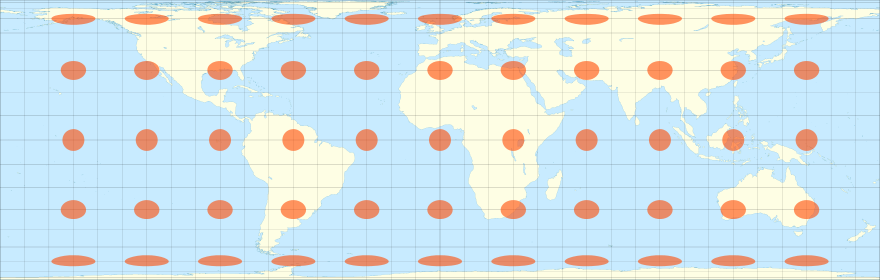
\includegraphics[width=\textwidth]{./Bilder/Lambert.png}
\caption{\label{fig_Lambert}%
Tissot-Darstellung der zylindrischen Lambert-Projektion. (Abbildunsquelle \cite{WikiLambert})}
\end{figure}

Abbildung \ref{fig_Lambert} zeigt eine zylindrische Lambert-Projektion der Erdkugel mit 
Tissot-Ellipsen.\index{Tissot-Ellipse!Lambert-Projektion}
Im Vergleich zu Abb.\ \ref{fig_Tissot1} f\"allt auf, dass die Ellipsen in Poln\"ahe nun flacher sind.
Die Ellipsen nehmen in der H\"ohe um denselben Faktor ab, um den sie in der Breite zunehmen.
Dadurch bleibt der Fl\"acheninhalt der Ellipsen \"uberall derselbe. Allerdings werden die Gebiete in
Poln\"ahe auch st\"arker in der H\"ohe zusammengepresst und im Vergleich zu einer formgetreuen
Darstellung verzerrt. Nun werden beide diagonalen Komponenten im metrischen Tensor an den Polen
singul\"ar.

\subsection{Die Mercator-Projektion}  
\label{sec_Mercator}

Obwohl man die Mercator-Projektion\index{Mercator-Projektion} 
als rechteckige Zylinderprojektion bezeichnet, handelt es sich
im strengen Sinne nicht um eine Projektion, da die Abbildung eines Punkts auf der Kugeloberfl\"ache
auf einen Punkt auf der Zylinderoberfl\"ache keine geometrische Konstruktion ist. Trotzdem besteht auch hier
die einzige Ver\"anderung zur quadratischen Zylinderprojektion in der Beziehung zwischen der
$y$-Achse und dem Breitengrad. 

Die Mercator-Projektion ist lokal winkel- und formtreu. Diese beiden Begriffe sind insofern
\"aquivalent, als aus lokaler Winkeltreue die lokale Formtreue folgt und umgekehrt: Wenn zwei
Dreiecke dieselben Winkel haben, haben sie auch die gleiche Form bzw.\ sind sich \"ahnlich, d.h., die 
Verh\"altnisse von je zwei Seitenl\"angen sind gleich. Die Mercator-Projektion ist nach Gerhard Mercator
(1512-1597)\index{Mercator, Gerhard} 
benannt, der diese Projektionen um 1570 zum ersten Mal f\"ur Weltkarten verwendete.
Die lokale Winkeltreue der Karte war fr\"uher in der Seefahrt von Vorteil, da ein bestimmter Kurs nach
dem Kompass (der den Winkel zu einem L\"angengrad angibt) einer geraden Linie entspricht. 
\"Uber gro\ss e Abst\"ande ist das aber nicht die k\"urzeste Verbindung zwischen zwei Punkten.
Gro\ss kreise (die die k\"urzeste Verbindung darstellen) werden auf Mercator-Karten nicht als
Geraden dargestellt. 

\begin{SCfigure}[30][htb]
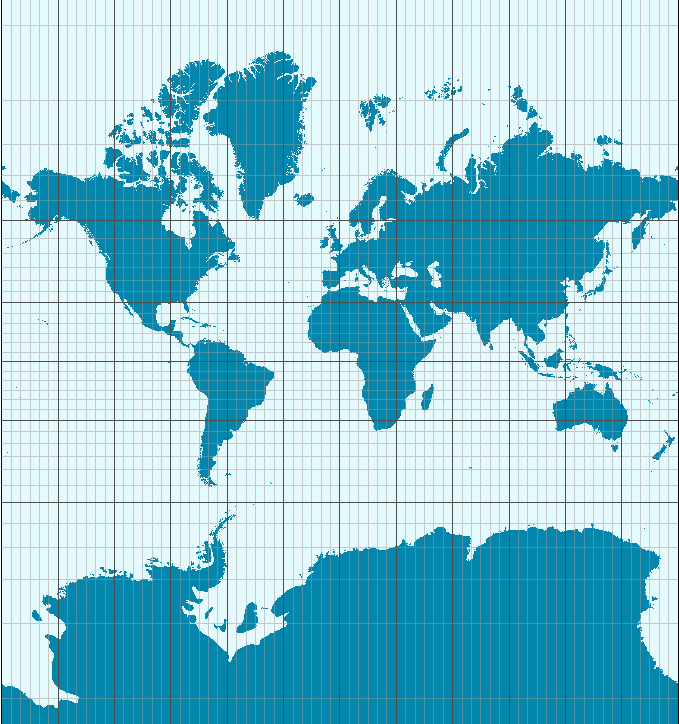
\includegraphics[trim= 0cm 1.0cm 0.3cm 1.0cm,clip,width=0.45\textwidth]{./Bilder/Mercator-proj.png}
\caption{\label{fig_Mercator}%
Eine Weltkarte in Mercator-Darstellung. In \"Aquatorn\"ahe gleicht diese Karte der
quadratischen Zylinderprojektion (Abb.\ \ref{fig_Zylinder}). Allerdings wird der Ma\ss stab in
Poln\"ahe nicht nur in die Breite sondern auch in die H\"ohe gestreckt. Dadurch erscheinen
die Umrisse von kleineren L\"andern zwar \"ahnlich wie auf einer lokalen Projektion, also
entsprechend ihrer lokalen Form, doch wirken
die L\"ander im Vergleich zu Gebieten am \"Aquator \"ubertrieben gro\ss. Afrika ist in Wirklichkeit
\"uber f\"unfzehnmal gr\"o\ss er als Gr\"onland, Australien ist viermal gr\"o\ss er. Afrika ist 
mehr als doppelt so gro\ss\ wie das Landgebiet der Antarktis. (Quelle \cite{WikiMercator})}  
\end{SCfigure}

Damit eine Karte formtreu ist, m\"ussen lokal die Abst\"ande in $x$-Richtung und in $y$-Richtung
um denselben Ma\ss stab ver\"andert werden, d.h., die beiden diagonalen Komponenten in der Metrik
sind gleich (aber ortsabh\"angig). Da wir bei der Parametrisierung nur die Beziehung zwischen dem
Breitengrad $\theta$ und der H\"ohe $y$ ver\"andern k\"onnen, ist eine Beziehung gesucht, sodass
\begin{equation}
     g = \frac{U^2}{B^2} \cos^2 \theta \left( \begin{array}{cc} 1 & 0 \\ 0 & 1 \end{array} \right)  
     \hspace{1cm} {\rm bzw.} \hspace{1cm}    \Delta \theta = \frac{2\pi}{B} \cos \theta\,  \Delta y \, .
\end{equation}
Zur Bestimmung von $y(\theta)$, der $y$-Koordinate auf der Karte als Funktion des Breitengrads,
haben wir somit das Integral
\begin{equation}
                     y(\theta) = \frac{B}{2\pi} \int_{0}^\theta \frac{1}{\cos \theta'} {\rm d}\theta'  
\end{equation}
zu l\"osen. Die L\"osung lautet:
\begin{equation}
                     y(\theta) = \frac{B}{2\pi}  \ln \sqrt{ \frac{1 - \sin \theta}{1+\sin \theta} }\, .
\end{equation}
Zur L\"osung des Integrals: Man erweitere den Integranden im Z\"ahler und Nenner um $\cos \theta'$, ersetze
im Z\"ahler $\cos \theta' \, {\rm d}\theta' = {\rm d} \sin \theta'$ und im Nenner $\cos^2\theta' = 1 - \sin^2 \theta'$.
Mit einer Partialbruchzerlegung, 
$\frac{1}{(1-\sin^2 \theta')} = \frac{1}{2} (\frac{1}{1-\sin \theta'} + \frac{1}{1+\sin \theta'})$
kann man das Integral leicht l\"osen. 

F\"ur kleine Werte von $\theta$, also in \"Aquatorn\"ahe, verh\"alt sich obige Beziehung wie in Gl.\ \ref{eq_Beztheta_z1},
aber f\"ur $\theta \rightarrow \frac{\pi}{2}$ divergiert dieser Ausdruck, d.h., der Nord- bzw.\ S\"udpol sind auf einer
Mercator-Karte im Unendlichen. Daher h\"oren die meisten Mercator-Karten auch etwas oberhalb des
$80$.\ Breitengrads auf (Abb.\ \ref{fig_Mercator} endet ungef\"ahr beim 83.\ Breitengrad) 

\section{Das UNO-Emblem}

\begin{SCfigure}[30][htb]

\includegraphics[trim= 0cm 1.0cm 0cm 1.0cm,clip,width=0.35\textwidth]{./Bilder/un_PNG20.png}
\caption{\label{fig_UN}%
Das Logo der Vereinten Nationen. In diesem Fall handelt es sich um eine sogenannte
Azimutalprojektion. Es wird eine Ebene an einen Punkt der Kugel gelegt (in diesem Fall
den Nordpol) und die Erdkugel wird in Polarkoordinaten um diesen Punkt herum dargestellt. 
Im vorliegenden Fall sind die Breitengrade von $90^\circ$-Nord bis rund $50^\circ$-S\"ud wiedergegeben.
Die Einteilung der Breitengrade ist in $30^\circ$-Schritten und die Breitengrade sind
\"aquidistant dargestellt. (Quelle \cite{UN})}  
\end{SCfigure}

Die Flagge der Vereinten Nationen (Abb.\ \ref{fig_UN})\index{Vereinte Nationen, Logo}
verwendet eine Darstellung der Erdkontinente in Polarkoordinaten - eine sogenannte 
Azimutalprojektion.\index{Azimutalprojektion}
In diesem Fall wird eine Ebene tangential an einen Punkt der Kugel gelegt (sehr h\"aufig, wie auch bei dem
UN-Logo, an den Nordpol) und die Kugeloberfl\"ache wird in Polarkoordinaten auf diese Fl\"ache
projiziert. Diese Darstellung (Nordpol als zentraler Punkt) wird auch hier gew\"ahlt.
Der Polarwinkel $\varphi$ entspricht dem L\"angengrad (allerdings wird im UN-Logo der
L\"angengrad $0$ nach unten projiziert). Die Breitengrade sind dann konzentrische Kreise um den
Nordpol. Der Abstand zwischen Breitengraden ist der einzige Freiheitsgrad, der hier gew\"ahlt
werden kann. Im UN-Logo sind die Breitengrade \"aquidistant angeordnet. Es gibt auch
fl\"achentreue Darstellungen, bei denen der Abstand zwischen Breitengraden von Nord nach
S\"ud abnimmt. Theoretisch gibt es auch eine konforme Abbildung, bei der die Fl\"achenform
erhalten bleibt, diese w\"urde sich aber nach Unendlich erstrecken und die L\"ander s\"udlich des
\"Aquators w\"aren \"ubertrieben gro\ss\ dargestellt. Azimutale Projektionen sind nur an einem
Punkt der Kugeloberfl\"ache singul\"ar, in diesem Fall am S\"udpol. 

Polarkoordinaten sind 2-dimensionale Koordinaten in der Ebene, gegeben durch\index{Polarkoordinaten}
\begin{equation}
          \pmb{x}(r,\varphi) = (r\cos \varphi, r \sin \varphi)  \, .
\end{equation}
(Wir w\"ahlen hier die \"ubliche Konvention, bei der $\varphi=0$ dem Punkt $(x,y)=(1,0)$ entspricht.
Die UN-Darstellung erh\"alt man aus der Koordinatenwahl $(x,y)=(r\sin \varphi, -r\cos \varphi)$.) Der
Winkel $\varphi$ entspricht direkt dem L\"angengrad. Der Breitengrad $\theta$ auf der Kugeloberfl\"ache
entspricht hier dem Radius, d.h.\ je nach Wahl der Darstellung ist $r=r(\theta)$ eine andere
Funktion. 

F\"ur Polarkoordinaten gilt die Beziehung:
\begin{equation}
           (\Delta s)^2 = (\Delta r)^2 + r^2 (\Delta \varphi)^2  \, .
\end{equation} 
Damit ist
\begin{equation}
     g =  \left( \begin{array}{cc} 1 & 0 \\ 0 & r^2 \end{array} \right) \hspace{1cm} {\rm bzw.} \hspace{0.7cm}
           (\Delta s)^2 = g_{rr} (\Delta r)^2 + (g_{r\varphi}+g_{\varphi r} ) \Delta r \Delta \varphi + g_{\varphi \varphi} (\Delta \varphi)^2  \, .     
\end{equation}
Wir erhalten diese Metrik wieder aus der Forderung
\begin{equation}
       g_{u u} = \frac{\partial \pmb{x}(u,v)}{\partial u} \cdot \frac{\partial \pmb{x}(u,v)}{\partial u} \hspace{0.7cm}
       g_{u v} = g_{v u} = \frac{\partial \pmb{x}(u,v)}{\partial u} \cdot \frac{\partial \pmb{x}(u,v)}{\partial v} \hspace{0.7cm}
       g_{v v} = \frac{\partial \pmb{x}(u,v)}{\partial v} \cdot \frac{\partial \pmb{x}(u,v)}{\partial v}   
\end{equation}
mit den Tangentialvektoren:
\begin{equation}
       \frac{\partial \pmb{x}(r,\varphi)}{\partial r} = (\cos \varphi, \sin \varphi) \hspace{1cm}
       \frac{\partial \pmb{x}(r,\varphi)}{\partial \varphi} = (- r\sin \varphi, r\cos \varphi)  \, .
\end{equation}

Wir m\"ussen nun noch die Beziehung zwischen $r$ auf unserer Karte (in Polarkoordinaten) und den
Breitengraden $\theta$ auf der Kugeloberfl\"ache herstellen. Die Winkel $\varphi$ sind in beiden F\"allen
gleich. Wenn wir den Durchmesser der Karte mit $D$ bezeichnen, entspricht $D$ einem Vollkreis, sodass
$r= D/(2\pi) \theta$. Umgekehrt entspricht auf der Erdkugel der Differenz von Breitengraden $\Delta \theta$ eine
Strecke von $\Delta l = R \Delta \theta = (U/2\pi) \Delta \theta$. Insgesamt erhalten wir somit:
\begin{equation}
                  \Delta r = \frac{D}{2\pi} \Delta \theta = \frac{D}{2\pi} \frac{2\pi}{U} \Delta l = \frac{D}{U} \Delta l \, , 
\end{equation}  
und misst man die L\"ange $l$ vom Nordpol aus zu einem Punkt auf der Erdkugel, gilt auch
$r=\frac{D}{U} l$. 

\section{Kuriosit\"aten}

\subsection{Tissot-Figuren in h\"oheren Dimensionen}

In drei Dimensionen wird eine\index{Tissot-Figur} 
Tissot-Figur zu einem Ellipsoid. Ein Ellipsoid ist gekennzeichnet durch
die drei Hauptachsen sowie die Lage im Raum (nochmals drei Winkel, d.h.\ sechs Parameter). Dies
l\"asst sich durch eine symmetrische $3\times 3$-Matrix $g_{ij}$ charakterisieren, sodass die Ellipsoid-Gleichung die Form
\begin{equation}
               (\Delta s)^2 = \sum_{i,j=1}^3 g_{ij} \Delta x_i  \Delta x_j    
\end{equation}
annimmt. Diese Gleichung bleibt unver\"andert auch in h\"oheren Dimensionen, lediglich die Indizes 
durchlaufen eine gr\"o\ss ere Indexmenge. Da $g$ symmetrisch (und damit selbst-adjungiert) ist, kann
man es durch eine Rotation diagonalisieren. Die Eigenwerte sind $\lambda_i=1/a_i^2$, wobei $a_i$ die
Hauptachsen des verallgemeinerten Ellipsoids sind, und die Rotation charakterisiert die Lage dieser
Hauptachsen im Raum.

\subsection{Tissot-Hyperbeln in Minkowski-R\"aumen}

In $(1+1)$-Raumzeit-Dimensionen handelt es sich bei den Tissot-Figuren um Hyperbeln und
die Vorgabe der Lichtkegelstruktur.\index{Tissot-Hyperbel} 
Die Kreisgleichung wird ersetzt durch
\begin{equation}
                          (\Delta t)^2 - (\Delta x)^2 = {\rm const.}   \, .
\end{equation} 
Ist die Konstante positiv, spricht man von\index{zeitartig}\index{raumartig} 
zeitartigen Ereignissen (die sich in ihrer
Lage um $\Delta t$ und $\Delta x$ unterscheiden). Ist sie negativ nennt man die Ereignisse
raumartig, und ist sie null, sind die Ereignisse lichtartig.\index{lichtartig} 
In diesen Koordinaten werden die
Lichtkegel durch Diagonalen dargestellt und die Skala ist in zeitartige und raumartige Richtungen
dieselbe. In einer allgemeinen Karte k\"onnen die Lichtkegel lokal gedreht sein und die Skalen
auch unterschiedlich. In h\"oher dimensionalen R\"aumen werden die Lichtkegel zu verallgemeinerten
Kegelmantelfl\"achen, die zeitartigen \glqq Hyperbeln konstanter Eigenzeiten\grqq\ werden zu
 \glqq Hyperbelschalen konstanter Eigenzeiten\grqq, die raumartigen Hyperbeln konstanter Abst\"ande
 werden zu Rotationsk\"orpern, die durch Drehung um die Zeitachse entstehen.

\subsection{Die Lambert-Karte und ein Theorem von Archimedes}

Eines der drei bekannten mathematischen Probleme der Antike war die geometrische Konstruktion --
nur mit Zirkel und Lineal -- eines Quadrats mit derselben Fl\"ache wie ein vorgegebener Kreis
bzw.\ letztendlich die Konstruktion der Zahl $\pi$ aus einer Einheitsl\"ange. Der Beweis, dass
dies nicht m\"oglich ist, erfolgte erst 1882 durch\index{Lindemann, Ferdinand} 
Ferdinand Lindemann. Genauer hat Lindemann
bewiesen, dass $\pi$ trans\-zendent ist (also keine L\"osung einer algebraischen Gleichung mit rationalen
Koeffzienten ist); dass sich transzendente Zahlen nicht geometrisch mit Zirkel und Lineal
konstruieren lassen, war schon vorher bekannt. 

Archimedes\index{Archimedes} 
konnte jedoch sehr viele Theoreme beweisen, bei denen krummlinige Fl\"achen
mit Quadraten oder Rechtecken in Beziehung gebracht wurden. Eines dieser Theoreme
besagt, dass die Oberfl\"ache einer Kugel genauso gro\ss\ ist wie die Mantelfl\"ache eines
Zylinders, der am \"Aquator um die Kugel gewickelt ist und dieselbe H\"ohe wie die Kugel hat. 
Heute w\"urden wir das folgenderma\ss en beweisen: Die Oberfl\"ache einer Kugel vom Radius $R$
ist $4\pi R^2$, ein um die Kugel gewickelter Zylinder hat die Grundseite $U=2\pi R$ (der Umfang
der Kugel) und die H\"ohe $2R$ und damit die Fl\"ache $2R\cdot 2\pi R = 4\pi R^2$. Manchmal
hei\ss t es auch, dass die Gesamtfl\"ache des umschriebenen Zylinders gleich $3/2$ mal
die Kugeloberfl\"ache ist: Die beiden Deckel haben zusammen eine Fl\"ache von $2 \cdot \pi R^2$; womit
man auch dieses Ergebnis leicht erh\"alt.   

\begin{SCfigure}[30][htb]
\begin{tikzpicture}
\draw (0.2,0.3) node{~};
\draw[thick] (2,2) circle (1.4 cm);
\draw[thick] (0.6,0.6) -- (0.6,3.4);
\draw[thick] (3.4,0.6) -- (3.4,3.4);
\draw[thick] (2,0.6) ellipse  (1.4cm and 0.2cm);
\draw[thick] (2,3.4) ellipse  (1.4cm and 0.2cm);
%\draw[thick] (6,1) -- (6,7);
\end{tikzpicture}
\caption{\label{fig_Archimedes}%
Die Archimedes-Figur. Angeblich wollte Archimedes, dass diese Figur auf seinem Grabstein abgebildet
wird. Dargestellt ist eine Kugel, die einem Zylinder gleicher H\"ohe eingeschrieben ist. 
Archimedes konnte beweisen, dass die Oberfl\"ache der Kugel gleich der Mantelfl\"ache des
Zylinders ist.} 
\end{SCfigure}

Angeblich wollte Archimedes auf seinem Grabstein die Figur aus Abb.\ \ref{fig_Archimedes} 
abgebildet haben, weil er die Beziehung zwischen der Kugeloberfl\"ache und der Mantelfl\"ache
des Zylinders als seine gr\"o\ss te Entdeckung ansah. Eigentlich hat Archimedes sogar mehr
bewiesen, als dass die Gesamtfl\"achen gleich sind; er hat bewiesen, dass kleine Ausschnitte
der Kugeloberfl\"ache, die man im Sinne der Lambert-Projektion von der Zylinderachse aus
auf die Zylinderfl\"ache projiziert, auf Fl\"achen derselben Gr\"o\ss e abgebildet werden. Damit
hat er die Fl\"achentreue der Lambert-Projektion bewiesen. 

Archimedes hat bei vielen seiner mathematischen Beweise sehr physikalisch gedacht und
oft infinitesimale Fl\"achen in Gedanken auf eine Balkenwaage gelegt und die Hebelgesetze
genutzt, um Beziehungen zwischen diesen Fl\"achen abzuleiten.  
Sehr oft kann man solche Operationen mit dem Strahlensatz und dem
Satz von den gleichen Verh\"altnissen von sich entsprechenden Seitenl\"angen in \"ahnlichen 
Dreiecken in Verbindung bringen. Der folgende Beweis nutzt nur diese beiden S\"atze.

\begin{figure}[htb]
\begin{tikzpicture}
\draw (0.0,0.0) node{~};
\draw (3,2.5) circle (2.5 cm);
\draw (0.5,0) -- (0.5,5);
\draw (0.5,2.5) -- (5.5,2.5);
\draw (3.0,0) -- (3.0,5);
\draw (0.5,3.8) -- (3.0,3.8);
\draw (0.5,4.2) -- (3.0,4.2);
\draw (3.0,2.5) -- (0.88,3.8);
\draw (0.88,2.5) -- (0.88,4.2);
\draw[thick] (0.52,3.8) -- (0.52,4.2);
\draw[thick] (2.98,3.8) -- (2.98,4.2);
\draw[thick] (0.88,3.8) -- (1.18,4.2);
\draw (0.4,4.0) node{${\scriptstyle h}$};
%\draw (3.13,4.0) node{${\scriptstyle h}$};
\draw (1.2,4.0) node{${\scriptstyle h'}$};
\draw (1.75,3.05) node{${\scriptstyle R}$};
\draw (2.0,3.7) node{${\scriptstyle R'}$};
\end{tikzpicture}
\hspace{1cm}
%
\begin{tikzpicture}
\draw (0.0,0.0) node{~};
\draw (5.5,5.0) arc (90:180:5cm);
\draw (0.5,0.0) -- (5.5,0.0);
\draw (0.5,0.0) -- (0.5,5.0);
\draw (5.5,0) -- (5.5,5);
\draw (0.5,2.6) -- (5.5,2.6);
\draw (0.5,3.4) -- (5.5,3.4);
\draw (5.5,0.0) -- (1.22,2.6);
\draw (1.22,0.0) -- (1.22,3.4);
\draw[thick] (0.52,2.6) -- (0.52,3.4);
\draw[thick] (5.48,2.6) -- (5.48,3.4);
\draw[thick] (1.22,2.6) -- (1.84,3.4);
\draw (0.4,3.0) node{${\scriptstyle h}$};
%\draw (5.63,3.0) node{${\scriptstyle h}$};
\draw (1.78,3.0) node{${\scriptstyle h'}$};
\draw (3.0,1.3) node{${\scriptstyle R}$};
\draw (3.5,2.45) node{${\scriptstyle R'}$};

\draw (5.55,0.0) node{${\scriptstyle A}$};
\draw (1.1,0.12) node{${\scriptstyle B}$};
\draw (1.1,2.72) node{${\scriptstyle C}$};
\draw (1.8,3.56) node{${\scriptstyle A'}$};
\draw (1.2,3.56) node{${\scriptstyle B'}$};

\end{tikzpicture}
\caption{\label{fig_Archimedes2}%
Zum geometrischen Beweis der Fl\"achentreue der Lambert-Projektion.
Die rechte Seite zeigt den Ausschnitt links-oben vergr\"o\ss ert. Da die Strecke
$A'C$ senkrecht auf $AC$ steht, sind die Dreiecke $ABC$ und $A'B'C$ \"ahnlich.
Daraus folgt $R'/R = h/h'$. 
} 
\end{figure}

In Abbildung \ref{fig_Archimedes2} (rechts) sind die beiden Dreiecke
$ABC$ und $A'B'C$ \"ahnlich. Das bedeutet: $h/h' = R'/R$. Stellen wir uns nun vor,
die infinitesimale Strecke $h$ auf dem Zylinder wird einmal um die zentrale
Zylinderachse rotiert, dann ist die \"uberstrichene Fl\"ache gleich $2\pi R h$. 
Die entsprechende Fl\"ache f\"ur das Streckenst\"uck $h'$ ist $2\pi h' R'$. Doch wegen
$h/h'=R'/R$ folgt, dass diese beiden Fl\"achen gleich sind. Diese Aussage gilt
nicht nur f\"ur den vollen Rotationsk\"orper, sondern auch f\"ur die \"uberstrichenen
Fl\"achen bei beliebig kleinen Rotationswinkel.\index{Landkarten|)}  


\begin{thebibliography}{99}
\bibitem{WikiNetz} Wikipedia \glqq Kartennetzentwurf\grqq:\\
    \url{https://commons.wikimedia.org/wiki/File:Zylinderprojektion_quadratische_plattkarte_kl.jpg}
\bibitem{WikiTissot} Wikipedia \glqq Tissot'sche Indikatrix\grqq:\\ 
       \url{https://de.wikipedia.org/wiki/Tissotsche_Indikatrix}
\bibitem{WikiLambert} Wikipedia \glqq Projection \'{e}quivalente cylindrique de Lambert\grqq;\\ 
    \url{https://upload.wikimedia.org/wikipedia/commons/thumb/c/cb/Tissot_indicatrix_world_map_Lambert_cyl_equal-area_proj.svg/880px-Tissot_indicatrix_world_map_Lambert_cyl_equal-area_proj.svg.png}
\bibitem{WikiMercator} Wikipedia \glqq Gerhard Mercator\grqq;\\ 
        \url{https://upload.wikimedia.org/wikipedia/commons/f/fa/Mercator-proj.png}
\bibitem{UN} UN-Logo:\\
            \url{https://pngimg.com/uploads/un/un_PNG20.png}

\end{thebibliography}

%\end{document}

